\section{Lineær spændingsregulator}\label{sec:lm317}
\begin{figure}[h!]
	\centering
	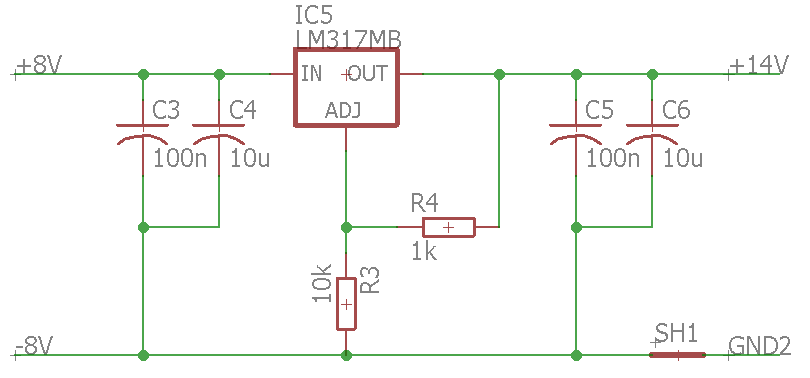
\includegraphics[width=.5\textwidth]{billeder/voltage_regulator.png}
	\caption{Diagram af spændingsregulator.}
	\label{fig:voltage_regulator}
\end{figure}
For at få en konstant spænding på $14\si{\volt}$ til frekvensgeneratoren, anvendes en LM317. Den har den fordel, at outputspændningen kan styres med kun to modstande. Det samlede kredsløb for spændingsregulatoren ses på figus \ref{fig:voltage_regulator}.
\subsection{Opstilling}
For at finde de to modstandsværdier anvendes ligning 1 fra databladet \cite[Side. 10]{LM317}.
\begin{align}
	V_{out} & = V_{ref} \cdot \left( 1 + \frac{R_3}{R_4} \right) + I_{ADJ} \cdot R_3 \label{eq:lm317_formel}
\end{align}
Hvor $V_{ref} = \SI{1.25}{\volt}$ og $I_{ADJ} = 100\si{\micro\ampere}$. Indsættes værdierne i formlen fås en outputspænding på $15\si{\volt}$. Grunden til, at spændingen bliver $15\si{\volt}$ og ikke $14\si{\volt}$ er adjust-ledet, $I_{ADJ} \cdot R_3$, som normalt kan negligeres, hvilket ikke er tilfældet her, da modstandsværdierne er for store. Vælges komponentværdierne $R_3 = \SI{3.3}{\kilo\ohm}$ og $R_4 = 330\si{\ohm}$ fås en outputspænding på $\SI{14.08}{\volt}$. Dog vælges der ikke at ændre komponentværdierne, dels fordi frekvensgeneratorens maksimale inputspænding er $16\si{\volt}$ og fordi komponenterne allerede var loddet på printet, da en ny beregning var foretaget.